\chapter{Base de données et administration}
\label{ch-bdd-admin}


\section{Conception}

\subsection{Les démarches de conception}

\par Les Acteurs : un acteur représente l’abstraction d’un rôle joué par des entités externes. Dans notre application on distingue principalement deux acteurs qui sont les suivant :

\begin{itemize}
\item Etudiant 
\item Administrateur
\end{itemize}

\subsection{Modèle conceptuel des données (MCD)}
 
\par Le modèle conceptuel des données a pour but de définir de façon formelle la structure de la base de données qui sera utilisée par le système d'information. Il s'agit donc d'une représentation du modèle de données, facilement compréhensible, permettant de décrire le système d'informations à l'aide d'entités. 
La figure suivante présente le modèle conceptuel des données.

\begin{figure}[H]
\centering
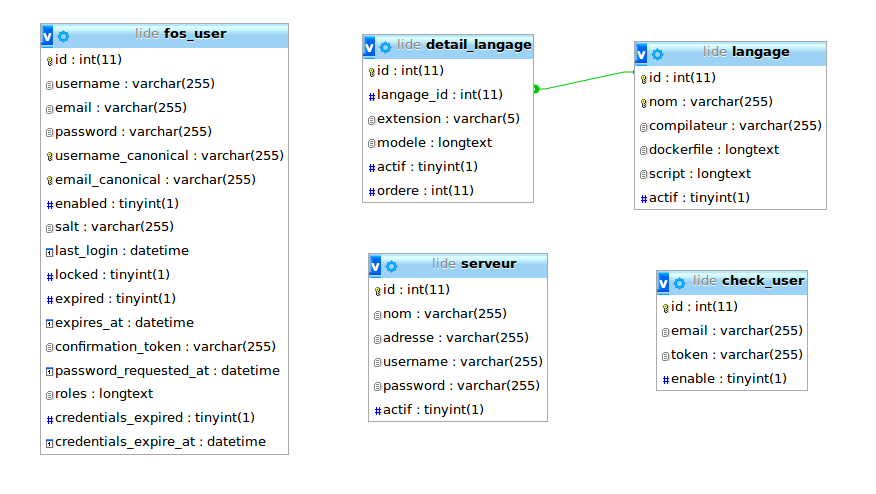
\includegraphics[width=0.8\textwidth]{./img/BDD.png}
\caption{Modèle conceptuel des données}
\end{figure}

\section{Base de données}

\subsection{Serveur}

\par La table serveur permettra de connaître les serveurs disponibles. Si il y a une surcharge, l’administrateur aura juste à ajouter un nouveau serveur et l’application pourra directement l’utiliser si besoin.

\subsection{Langage}

\par Le nom d’un langage est UNIQUE. La table langage contient le dockerfile permettant d’installer le nécessaire pour pouvoir compiler/exécuter le langage. Il y a aussi le script qui permet de lancer la compilation avec les fichiers de l’utilisateur. Pour finir, il y a le compilateur. 
L’avantage de stocker en base de données les langages est de rendre autonome les enseignants. S’ils veulent rajouter un nouveau langage, il leur suffit de l’ajouter avec son dockerfile et son script.

\subsection{Détails langage}

\par La table details\_langage contient les extensions du langage correspondant ainsi qu’un modèle de base (par exemple le Hello World). Cela permet de proposer à l’utilisateur l’extension qu’il veut écrire.
Toutes les trois tables contiennent un champ actif qui permet d’activer ou de désactiver le tuple. Par exemple si un serveur est en maintenance ou ne doit pas être utilisé, il pourra être désactivé et réactivé au besoin par l’administrateur. C’est la même chose pour la table langage et details\_langage.

\subsection{Fos user}

\par Dans cette table on sauvegarde tous les informations des utilisateurs.
check\_user: 
Cette table est pour but de sauvegarder les emails des utilisateurs  qui n’ont pas confirmer encore leur inscription par  le lien de validation reçu dans leur boite mail. 

\subsubsection{FOSUserBundle}

\par Ce bundle nous a permet de gérer assez facilement les utilisateurs  inscription, connexion, droits d’accès, etc…

\subsubsection{EasyAdmin}

\par Ce Bundle nous a permet de créer facilement l’interface administrateur.